\phantomsection
\refstepcounter{dummy}
\addcontentsline{toc}{chapter}{\tocEntry{Introduction}}

\chapter*{Introduction}

\renewcommand{\thefigure}{\Alph{figure}}

\begin{epigraphs}
\qitem{
[...] \textnorsk{og fordi jeg alltid har hatt en dragning mot det skjulte og hemmelige.}
}{
--- \textnorsk{\textsc{K. O. Knausgård}, \textit{Om Høsten}}}
\end{epigraphs}


\section*{What Are the Electrons Really Doing in Molecules?}

This question was posed by R.~S.~Mulliken over a half-century
ago\footnote{This was the title Mulliken chose for his Gilbert N.~Lewis
award acceptance speech in 1960.}
and can be considered the fundamental research question behind the
development of quantum chemistry.
The purpose of quantum chemistry is to provide models based on first
principles that can help \emph{understand} and \emph{predict} molecular properties.
As stated by \citeauthor{Dirac1929-gn} in his \citetitle{Dirac1929-gn}
paper:\autocite{Dirac1929-gn, Kutzelnigg2000-fl}
\blockquote{The underlying physical laws necessary for the mathematical
theory of a large part of physics and the whole of chemistry are thus
completely known, and the difficulty is only that the exact application of
these laws leads to equations much too complicated to be soluble. It
therefore becomes desirable that approximate practical methods of
applying quantum mechanics should be developed, which can lead to an
explanation of the main features of complex atomic systems without too
much computation.}
Following Dirac's \emph{dictum}, in quantum chemistry we apply physical
models based on quantum many-body methods to molecular systems, employ
their mathematical realizations and devise computable approximations.
The central idea is, in fact, to be able to obtain an algorithmic
implementation of the methods that can be applied to interesting
chemical systems: model building and software implementations are two
closely intertwined aspects in the practice of quantum chemistry.

\begin{figure}[tb]
\centering
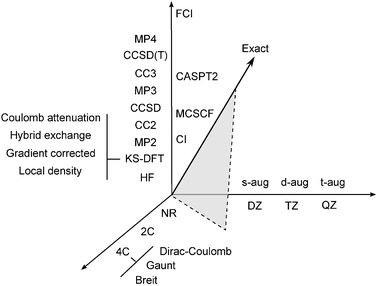
\includegraphics[width=.6\textwidth]{qc-axes.png}
\caption[Pictorial depiction of the concept of \emph{model chemistries}.]{
Pictorial depiction of the concept of \emph{model chemistries} as the
three dimensions of quantum chemistry.\autocite{Pople1999-gt, Saue2011-qg}
Reproduced from \noparcite[ref.][]{Norman2011-ad} with permission from the PCCP Owner Societies.
}
\label{fig:RQC-axis}
\end{figure}

It is easy to manipulate chemicals in a virtual laboratory. Nowadays
quantum chemical methods often complement traditional experimental
approaches. They have become invaluable tools in the modern development
of chemistry,\autocite{Lee1995-pw, Helgaker2004-oz, Tajti2004-ye} as
witnessed by the Nobel prizes awarded in 1998\autocite{Nobel1998} and
2013.\autocite{Nobel2013}
The concept of \emph{model chemistries} is at the heart of these
successes. Introduced by \citeauthor{Pople1999-gt}, theoretical model
chemistries are specific combinations of approximations in the basis set
and molecular electronic structure methodology.\autocite{Pople1999-gt}
Model chemistries are \emph{systematically improvable} so that it is
possible to achieve the heaven of chemical accuracy by relaxing
approximations in the model, albeit at an increased computational cost.
Figure \ref{fig:RQC-axis} presents the usual depiction of this concept
as a set of orthogonal axes, where chemical accuracy can be achieved by
moving away from the origin.
Relativity can be considered as the third axis of quantum
chemistry: accuracy can be reached improving on the Hamiltonian, method
and basis axes.\autocite{Saue2011-qg}

The description of the ideas and methods at the basis of quantum
chemistry will be the subject of Chapter \ref{ch:QM}.
I will put emphasis on the methods that have been relevant in the work
presented in this thesis. Section \ref{sec:mqm} discusses some of the
ideas of quantum many-body theory relevant to quantum chemistry. Section
\ref{sec:mean-field} introduces the workhorses of quantum chemistry
\acrlong*{HF} and \acrlong*{KS} \acrlong*{DFT}.
The \acrlong*{MBPT} and \acrlong*{CC} rungs on the methodology axis will
be discussed in Sections \ref{sec:mbpt} and \ref{sec:coupled-cluster},
respectively.

\section*{The Problem of Solvation or Taming Complexity with Models}

Chemistry can be largely considered a \emph{wet} science: almost always
chemical phenomena happen in a liquid environment.\autocite{Reichardt2010-le}
We hereby define a "solution", or more generally an "environment", as
a system where the number of solvent molecules exceeds by far the number
of solute molecules.\autocite{Tomasi2004-dc, Tomasi2007-es}
It is then clear that theoretical and computational approaches to such a
problem will necessarily suffer from a \emph{dimensionality disease}.
The number of degrees of freedom to be taken into account is, in
principle, so large, that even the most advanced computing machines
would have a hard time computing the desired observables.
Moreover, on an interpretive level, it would not even be desirable to
have such a detailed insight.
As is well known from statistical mechanics, microscopic detail cannot
account for the macroscopic behaviour.\autocite{Hill1960-ql,
Hansen2013-io}
To tame this complexity and cure the disease, one must devise
\emph{models} that simplify physical reality, while offering tools for
understanding reality and predicting new and exciting
phenomena and properties.\autocite{Anderson1972-ai, Winsberg2010-sy, Kovac2011-ew}
One of the earlier attempts at tackling the problem of solvation is due
to \citeauthor{Onsager1936-wf}. His was a rather crude model, but one
that has had a lasting impact and informs much of the developments that
will be presented in this thesis.\autocite{Onsager1936-wf}

Before introducing our model of choice, let us consider how an
environment might affect molecular observables of interest.
Environment effects are usually classified as:
\begin{description}[font=\normalfont\scshape]
\item[Direct.]
  These effects stem straightforwardly from the modification underwent by
  the solute electronic density when interacting with the environment.
\item[Indirect.]
  It is common for solutes to exhibit different minimum-energy
  conformations in different environments. These effects are commonly
  labelled as indirect.
\item[Local field.]
  Light-matter interactions are also affected by the environment. Local
  modifications of externally applied fields subtly influence molecular
  responses.\autocite{Cammi1998-jp, Pipolo2014-sd}
\item[Dynamic.]
  Probing the nature of molecular excited states has enormous
  technological impact. The presence of the environment radically
  influences excited states, since relaxation processes in the medium
  become important.
\item[Specific.] This catch-all category includes all effects
  stemming from the peculiar solute-solvent pair interactions that
  cannot be fully described under any of the previous labels.
  In general, modelling such effects demands an atomistic level of
  detail.
\end{description}

Faced with the problem of describing such a diverse array of effects,
two main models have emerged in the past decades, each with its
strengths and weaknesses.
Both can be classified as \emph{multiscale} (or \emph{focused})
models\autocite{Nobel2013} and hinge on the same idea: treat different
parts of the system with different methods and couple these methods by
bridging "scales" at the boundary.
Figure \ref{fig:qm-to-multiscale} schematically portrays the transition
from a full \acrshort{QM} model of the relevant system to its multiscale
representations.

\begin{figure}[tb]
\missingfigure{Add picture with multiscale models}
\caption[From quantum mechanical to multiscale models]{
From quantum mechanical to multiscale models.
The images used in the scheme are reproduced courtesy of Dr.~Stefano
Caprasecca (MoLEcoLab, Università di Pisa).}
\label{fig:qm-to-multiscale}
\end{figure}

While both models treat the molecular degrees of freedom at the quantum
mechanical level, their approach to the microscopic description of the
degrees of freedom of the environment differs:
\begin{itemize}
 \item
   \emph{Discrete} (or \emph{explicit}) models explicitly treat those
   degrees of freedom.
   This is either achieved by a cheaper quantum mechanical
   method\autocite{Vreven2006-gx} or by \gls{MM}.\autocite{Senn2009-sk}
   In the latter approach, commonly dubbed \acrshort{QM}/\acrshort{MM}, the \acrshort{MM}
   region can either be polarizable\autocite{Mennucci2013-go,
   Olsen2010-wa, Lipparini2011-rd} or non
   polarizable. While the former method allows for mutual polarization
   between the \acrshort*{QM} and \acrshort*{MM} subsystems, the latter
   treats the \acrshort*{MM} region as fixed.
 \item
   \emph{Continuum} (or \emph{implicit}) completely remove the degrees
   of freedom of the environment from the model, replacing them with a
   structureless continuum.
   The effect of this continuum is described, classically, \emph{via}
   its bulk properties.\autocite{Onsager1936-wf, Miertus1981-mm}
\end{itemize}

\acrshort{QM}/\acrshort{MM} models can capture, albeit approximately, the effect
of the atomistic nature of the environment on the active part of the
system.
However, they demand a statistical average of environment configurations
to yield results of any significance. Moreover, a rather large
\emph{cutoff radius} for the \acrshort{MM} region is usually required to converge
long-range electrostatic interactions.\autocite{Steindal2011-ki}
Continuum models avoid both problems at once. Statistical averaging is
built into the model \emph{via} their parametrization by
means of the environment's bulk properties, such as the permittivity.
In addition, long-range electrostatics is treated exactly.
Unfortunately, atomistic detail is lost and it is then impossible to
recover a satisfactory description of specific effects.
To partly alleviate these sources of error, the
\acrshort{QM}/\acrshort{MM} and \acrshort{QM}/Continuum methods can and
have been successfully combined to yield the three-layer
\acrshort{QM}/\acrshort{MM}/Continuum method.\autocite{Steindal2011-ki,
Lipparini2011-rd, Caprasecca2012-ir, Lipparini2013-ud}

Notice that we have deliberately ruled out so-called \emph{cluster}
models from the above discussion.
These approaches replace the actual physical setting with a suitable
truncation of the whole solute+solvent system, the \emph{model system}
and treat it within a chosen quantum mechanical level of theory.
Cluster models can be used to benchmark more approximate multiscale
models, but their description is outside the scope of this thesis.

Chapter \ref{ch:CSM} will present an overview of the \gls{PCM} for
solvation.
I will present a nontechnical discussion of the mathematical details of
the model and an outline of current methodologies for the solution of
the associated governing equations.
Borrowing from the work of \citeauthor{Lipparini2010-be},\autocite{Lipparini2010-be,
Lipparini2015-lq} I will introduce a unifying theoretical formalism for
\acrshort{QM}/Continuum, \acrshort{QM}/\acrshort{MM} and \acrshort{QM}/\acrshort{MM}/Continuum models that will
be extensively used throughout the thesis.

\section*{The Road to Reality or Molecular Response Properties}

The scope of quantum chemistry is to understand and predict molecular
properties, but so far we have made no mention of properties other than
the energy.
The experimentalists' view of molecular systems is built mainly around
the use of spectroscopic techniques that explore the interaction of
light and matter. When a system is exposed to an external perturbing
electromagnetic field, it will respond with a detectable change in its
properties.\autocite{Pedersen2012-il, Jaszunski2012-wy}
Characterizing, explaining and predicting a large number of measurable
properties requires a synergistic experimental and theoretical approach.
\emph{Response theory} is the missing link between theory and
experiment, making quantum chemistry a full-fledged virtual laboratory.
Response theory allows the description and computation of
perturbation-induced changes in observable molecular properties.
Electric and magnetic properties, excitation energies and transition
moments can easily be calculated in the framework of response theory.
\emph{Response functions} are the central concept in response theory.
These are built solely by means of \emph{unperturbed} molecular states and
energies: no explicit modelling of excited states is needed.

Response theory will be the subject of Chapter \ref{ch:molprop},
where the basic ideas in the computation of response functions will be
presented. We will discuss the formulation of the linear response
function for quantum/classical polarizable Hamiltonians and show how the
variational framework is a powerful theoretical tool.

\section*{Accurate Methods for Accurate Properties}

The concepts of systematic improvability and theoretical model
chemistries are the foundations for the successful practice of quantum
chemistry.
A balanced description of electron correlation is often necessary
to achieve accurate enough results in the computation of molecular
properties.\autocite{Lee1995-pw, Helgaker2004-oz, Tajti2004-ye}
The cost-effective treatment of electron correlation is a challenging
problem and a very active line of research in the field.
\Acrlong*{DFT} approaches are cheap and widespread, but their general
accuracy is hard to assess. \Acrlong*{MBPT} and \acrlong*{CC} approaches
are more robust in this respect, albeit at an increased computational
cost.

In this thesis, we are interested in the inclusion of
environment effects in \emph{ab initio} models of interesting chemical
systems. As already noted, this is a challenging problem, the more so
when including electron correlation is necessary to obtain better
accuracy.
We will describe our approach to this problem in Chapter
\ref{ch:solvation-correlation}. Treating solvation and electron
correlation has been a recurring subject of research in the literature
since the inception of continuum models. Once again, we will leverage
the variational formulation of classical polarizable models presented
in Chapter \ref{ch:CSM}.
